\chapter{Learning user preferences in object placement}


As robots achieve long term autonomy and they intend to stay longer in human environments, they should be able to adapt quickly to the corresponding environments and the user. Since they are service robots its acceptable for a new robot to ask for help from its user in the initial days it moves to a new home, for eg. Where to find a cup?. But as the robot stays longer in a home it becomes less acceptable that the robots ask the user for the same questions, i.e. they should have the capabilities to learn from previous information provided by the user. Also it should be able to reason and learn from its own the previous observations of the user or environment to generate new knowledge about the user or environment. For example, the robot can learn about the user preferences in the cutlery used to setup a breakfast table from previous days observations of breakfast tables. In this chapter we look at such one example of knowledge generation based on previous observations, for learning the user preferences in object placement.

The main advantage of learning user preference would be in object search. In classical object search, the search is based on the knowledge of object locations in a generic home (For eg: cups are found in kitchen, books in shelves). Thus these generic home knowledge based classical object search doesn't take into account the differences in object locations from home to home. Based on practical experience we know that the even though homes have same base structure in space but the usage of the space is based on the user preferences. Each home is different from other home because of the humans which reside in them use it according to their likes (For eg: some users the keep books on the study table). The proposed model will try to learn these user preferences in each home. So rather than learning object locations in a generalized home the proposed model shall learn object locations in a specific home.


\begin{figure}[htp]
\centering
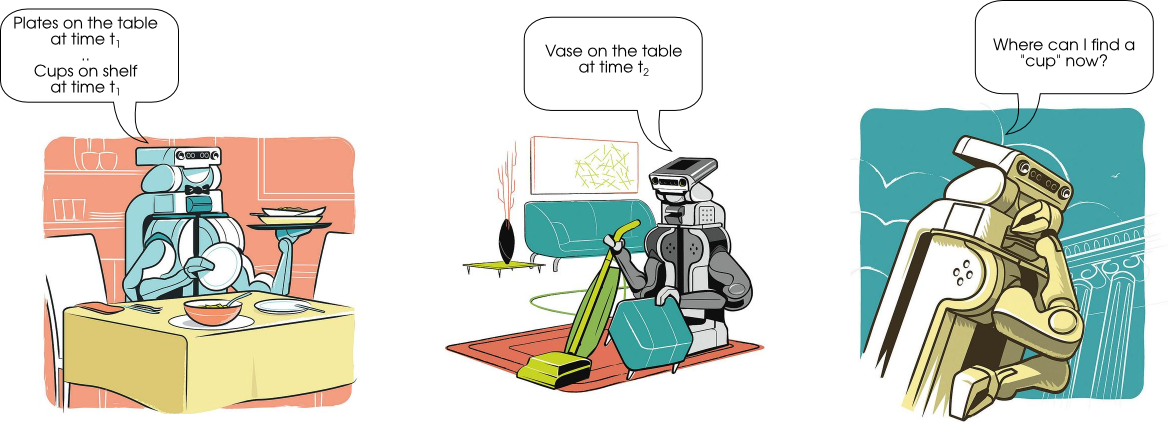
\includegraphics[scale=0.4]{pictures/scenario.png}
\caption{Robot recording perceived objects location and time. Based on the
recordings robot making prediction on the location of the cup for current time
Images courtesy : \url{https://www.flickr.com/photos/willowgarage} }
\label{scenario}
\end{figure}

Consider a domestic robot which has been placed in a home environment with a known map
and semantic information of the different locations in the home. The domestic robot while doing its daily activities 
makes a record of the objects seen in the environment with
their location and time. Now the robot has been asked to bring the coffee mug
of the user.
The robot has to make a decision which part of the home it has to go to look for
the coffee mug.
The robot can make this decision based on the previous observations of the 
location of the coffee mug.
The robot using the previous observations and the time of those observations 
makes a prediction about where the coffee mug can be found at the current time.
Based on previous observation it can be
inferred that the coffee mug is usually found in any of the following three location
dishwasher/platform/cupboard. Assuming that the time now is morning, from
previous observations it can be found that the coffee mug was always found  in the
dishwasher. The above example illustrate the main aspects of object location
prediction we wish to capture in this chapter.


The model needs to capture two main
elements; first that objects in a human environment are not placed randomly but
usually have a certain set of places where they are placed.
These places of object placement differ from home
to home. These object locations entirely depends on the users preferences.  
Second, that human behaviour is related to time i.e. Humans have daily routines  and the object locations are influenced by these routines.
Thus human behaviour not only  has a spatial behaviour but also has a temporal behaviour.
The model will reason on both user preference of the object placement and the
object-time relation.

\section{Beta-Bernoulli model}


Beta Bernoulli model is a two-level Bayesian model. The basic idea is that observations of all the objects at each location, each time period is characterized by a distribution.

The data are the boolean observation of the object at a location $x_{ij}$ for $i = 1 \dots T$ time periods and then $j = 1, \dots , N$  are the observations.  We assume that the latent pattern for finding the user to place the object at a  location in a particular period can be represented as a Bernoulli distribution. The number of periods $T$ for our model is fixed to 24 corresponding to the number of hours in a day. 

The conjugate prior for the Bernoulli distribution is the Beta distribution. The model estimates the posterior distribution of $\theta_i$ given our current data and prior beliefs. Our prior beliefs are encoded in the model through the prior $\alpha$ and $\beta$, which represents pseudocounts of what we believe the data should look like – currently taken as same values representing no prior information. The probabilistic graphical model is shown in Figure \cite{bbm}


\noindent
\begin{figure}[htp]

\begin{minipage}{0.3\textwidth}
\centering

\tikz {
 % Define nodes
  \node[latent]                                 (theta) {$\theta$};
  \node[latent, above=of theta, xshift=-1.2cm]  (alpha) {$\alpha$};
  \node[latent, above=of theta, xshift=1.2cm]   (beta) {$\beta$};
  \node[obs, below=of theta]                    (y)     {$y$}; 
  % Connect the nodes
  \edge {alpha,beta} {theta} ; %
  \edge {theta} {y};
  % plates
  \plate {location} {(y)} {location};
  \plate {time} {(theta)(y)(location)} {time};
}

\end{minipage}%
\begin{minipage}{0.7\textwidth}

\begin{equation*}
	\alpha = 2 ; \beta = 2;
\end{equation*}
\begin{equation*}
	\theta \sim Beta(\alpha, \beta);
\end{equation*}
\begin{equation*}
	y = Bernoulli(\theta)
\end{equation*}
\end{minipage}
\caption{Graphical model representation of Beta-Bernoulli model. The boxes are ``plates" representing replicates. The outer plates represents hours of a day, while the inner plate represents the observed locations within each hour.}
\label{dcm}
\end{figure}

\section{Hierarchical Beta-Bernoulli model}

\section{Evaluation}

\section{Discussion}